\begin{savequote}[75mm]
Framing reality is one of the only ways we can be sure it exists.
\qauthor{Sturgill Simpson}
\end{savequote}

\chapter{ATLAS Computing and Software}

\newthought{The ATLAS Detector produces petabytes of data every year while ATLAS researchers produce additional petabytes of simulated data for validation studies and analysis design.} The production, processing, and analysis of this data requires massive computing resources and the development specialized software. The ATLAS data ecosystem is described in the following chapter and is summarized in Figure \ref{fig:data_flow}.

\begin{figure}[h]
    \centering
    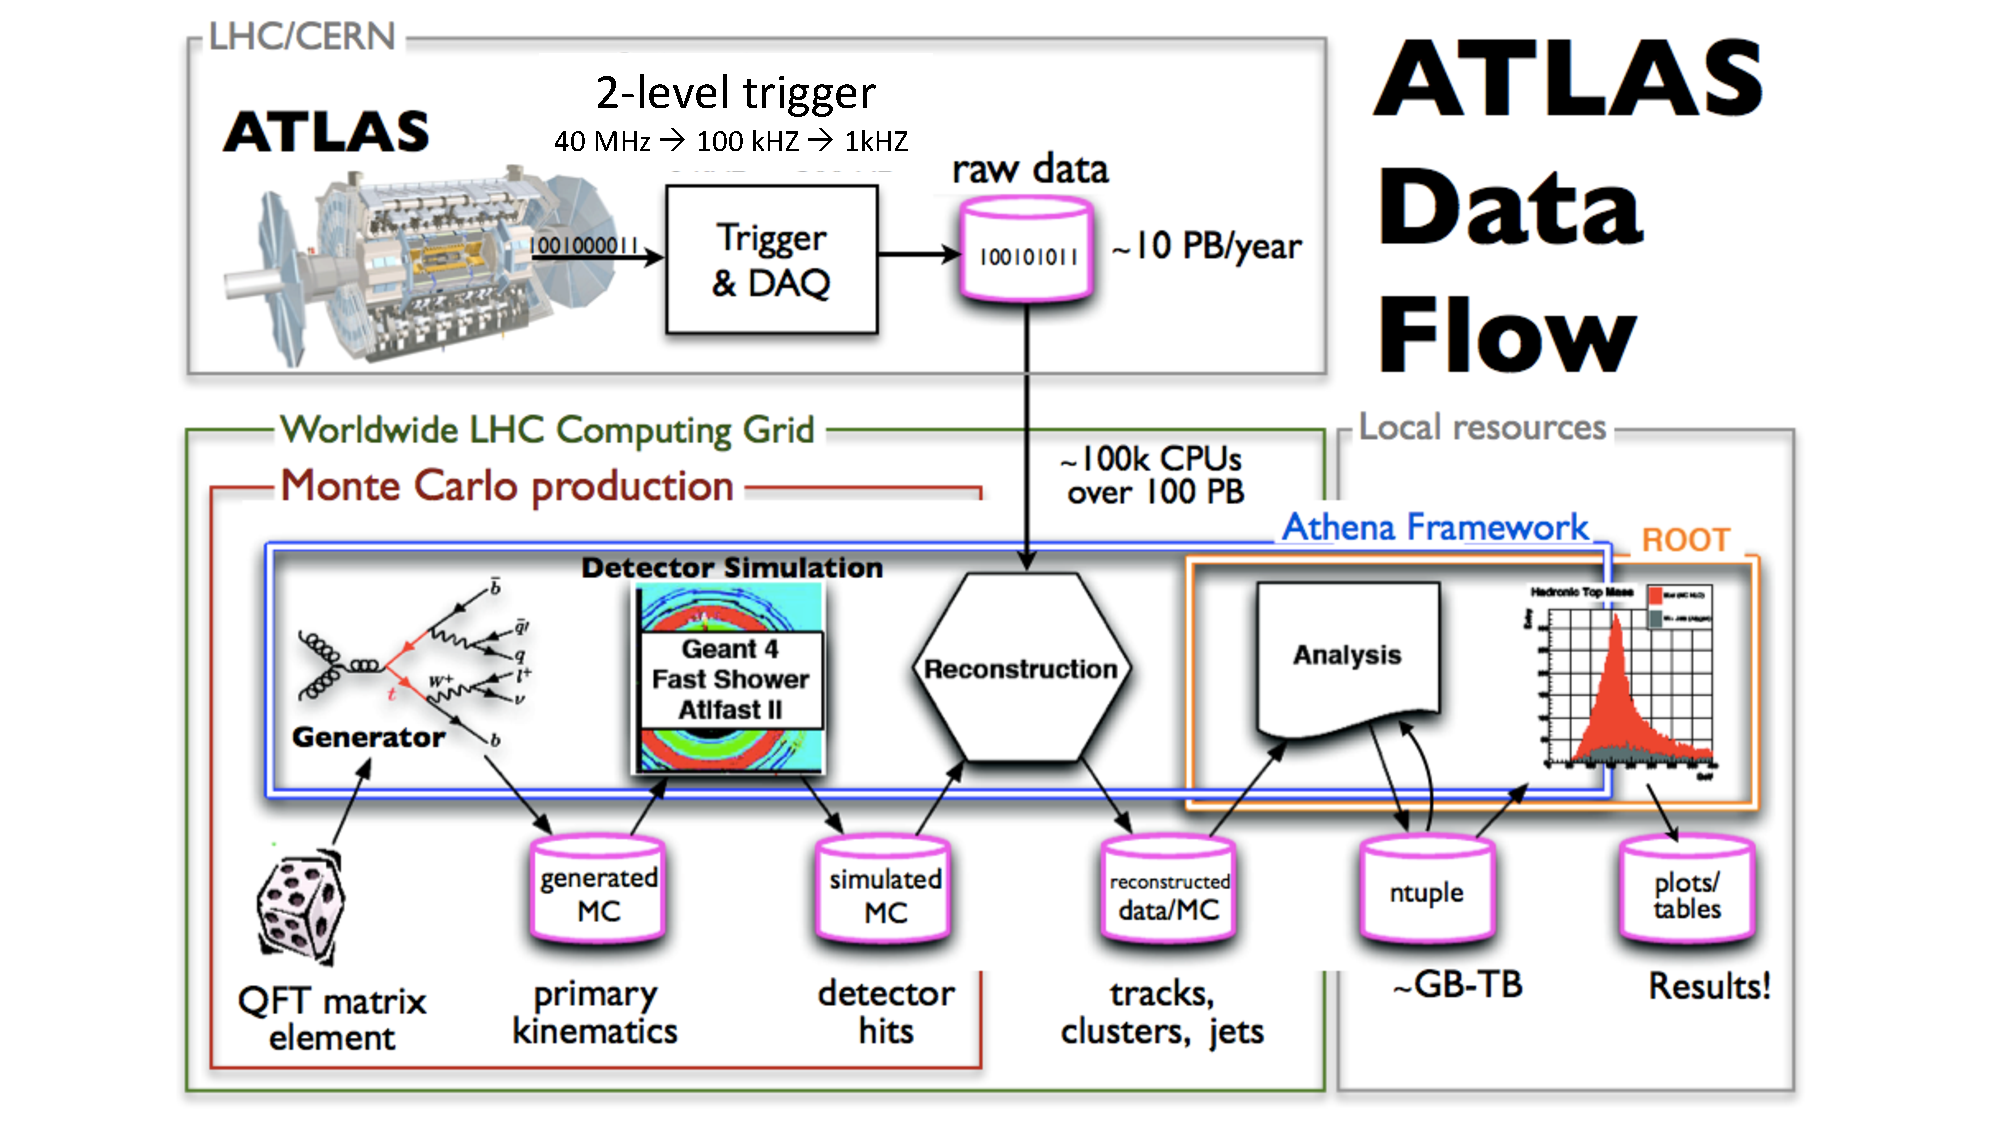
\includegraphics[width=5in]{figures/chapter3/atlas-data-flow.pdf}
    \caption{A high-level summary of the ATLAS data flow \cite{data_flow}.}
    \label{fig:data_flow}
\end{figure}

%% SEC: DAQ AND STORAGE
\section{Data Acquisition and Storage}
The first stage of processing for collision data is the Trigger and Data Acqusition System, collectively referred to as TDAQ. When the LHC is running at optimal performance, it produces over 30 million bunch crossings per second within the ATLAS detector. Each physics event requires approximately 25 megabytes to store the information from all readouts; this corresponds to a data production of nearly 60 million GB per second which, given current technology is impossible to store without some sort of size reduction \cite{trig_web}. Furthermore, as described in Chapter 2, a large portion of the data does not correspond to the hard-scattering events of interest. Thus, ATLAS relies heavily on the trigger system, a 2 level computing system which selects 0.1\% of events for storage and further analysis \cite{trig_2015}.\\

%%subsec: trigger and DAQ
\subsection{Triggers and DAQ}
The ATLAS TDAQ is divided into 2 distinct levels as shown in Figure \ref{fig:trig_diag}. The Level 1 Trigger (L1), a hardware trigger which uses a subset of information from the calorimeters and muon spectrometer, and the software-based High Level Trigger (HLT), which refines L1 decisions by applying reconstruction algorithms that closely mirror the offline algorithms while accounting for trigger specific time and CPU constraints \cite{trig_2015}.\\

\begin{figure}[h]
    \centering
    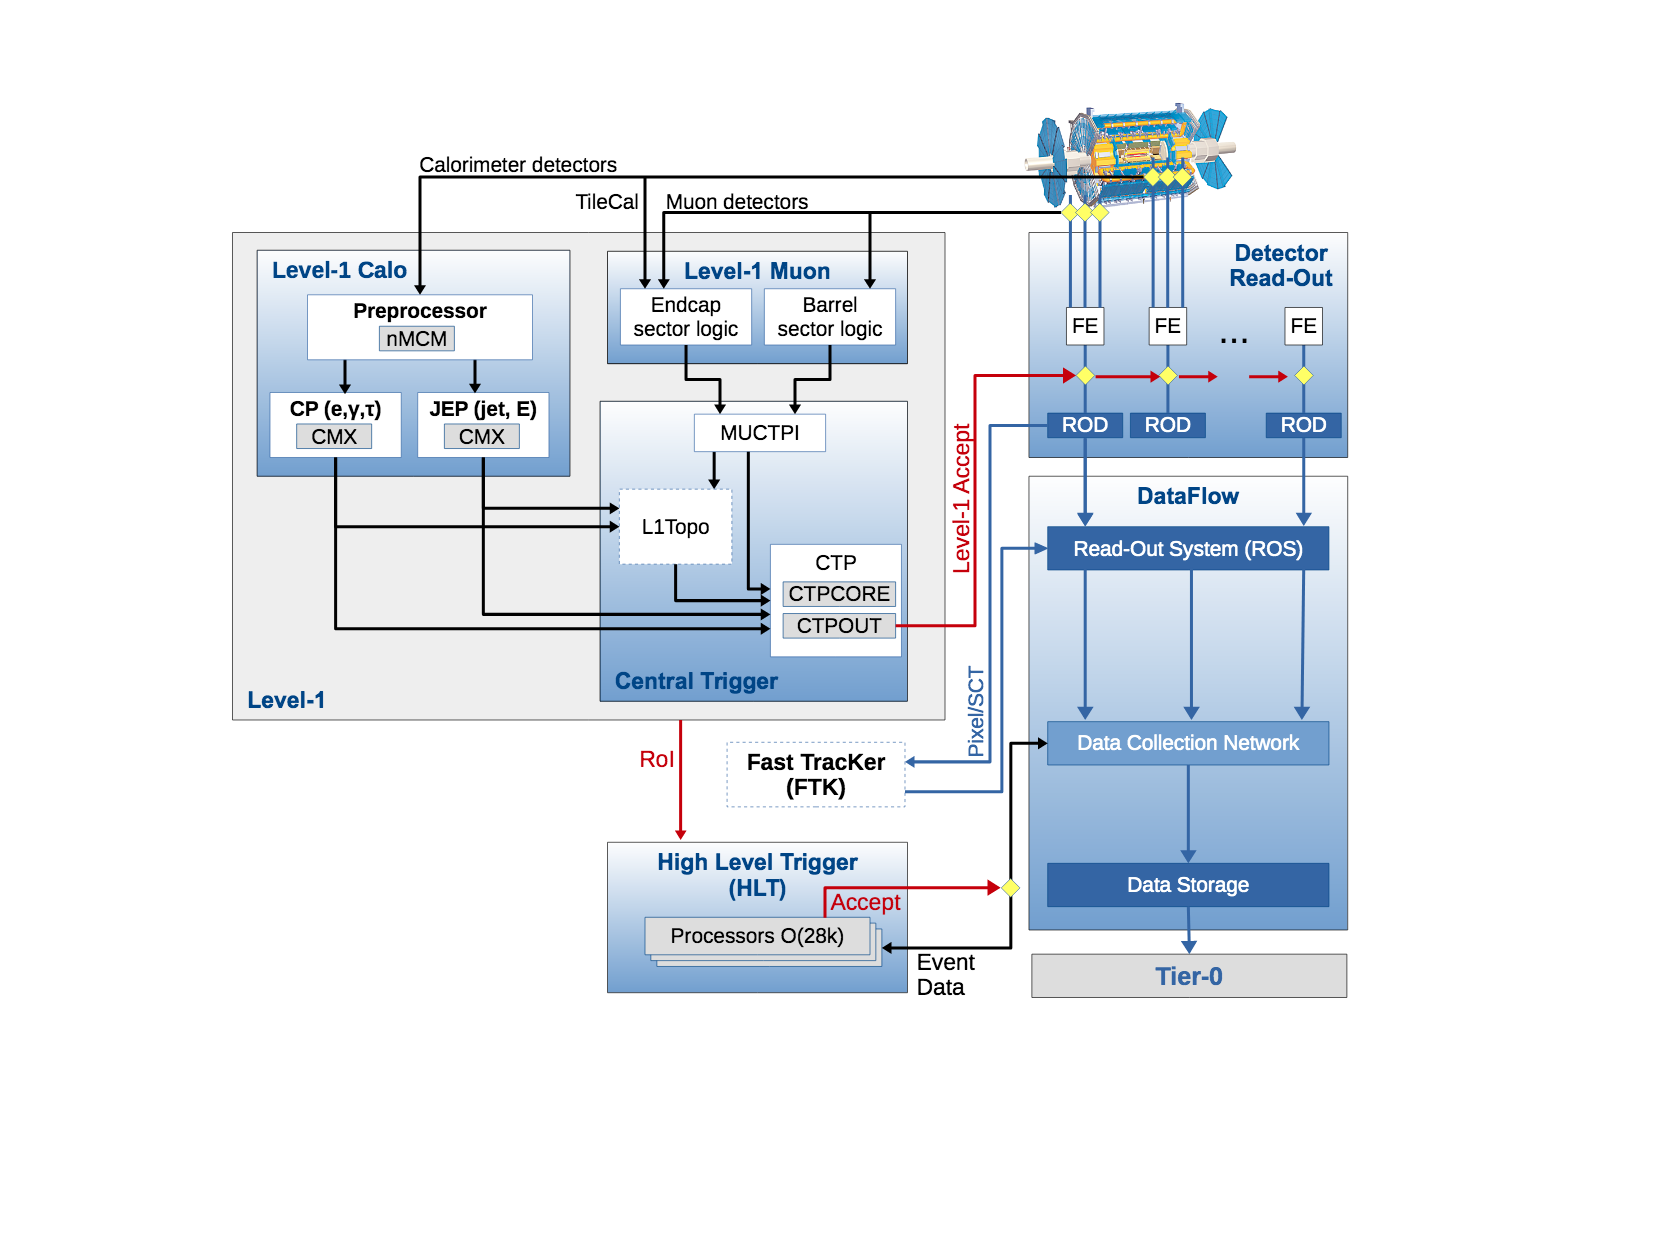
\includegraphics[width=5.5in]{figures/chapter3/trig_diag.pdf}
    \caption{Schematic diagram of the ATLAS TDAQ System in Run 2. The FTK is still in the commissioning phase \cite{trig_2015}.}
    \label{fig:trig_diag}
\end{figure}

The L1 trigger runs on custom FPGAs (Field Programmable Gate Arrays); decisions are completed within 2 $\mu$s of the event occurring and it has a total output frequency of less than 100kHz. The final L1 decision is determined by the central trigger processer (CTP) which receives information from the calorimeters and muon spectrometer, as well as information from Minimum Bias Trigger Scintillators, the LUCID Chernekov Counter, and the Zero-Degree Calorimeter \cite{atlas}. The L1 calorimeter algorithms utilize Region of Interests (ROIs) formed from trigger tower clusters (Figure \ref{fig:l1calo}) whose energy exceeds a predefined threshold. ROIs for EM objects and taus are formed and processed separately from ROIs for jets, and this information is merged in the L1Topo module and sent to the CTP. The L1 muon algorithms relies on signals from the muon trigger chambers. Information from the barrel and endcap chambers are processed separately to find hit patterns consistent with high-$p_T$ muons originating from the interaction point and these signals are then combined and passed to the CTP. The CTP implements a trigger `menu' of different combinations of object types and energies, and surviving events are then buffered in the Read Out System (ROS) and eventually sent to the HLT \cite{trig_2015}.\\

\begin{figure}[hb!]
    \centering
    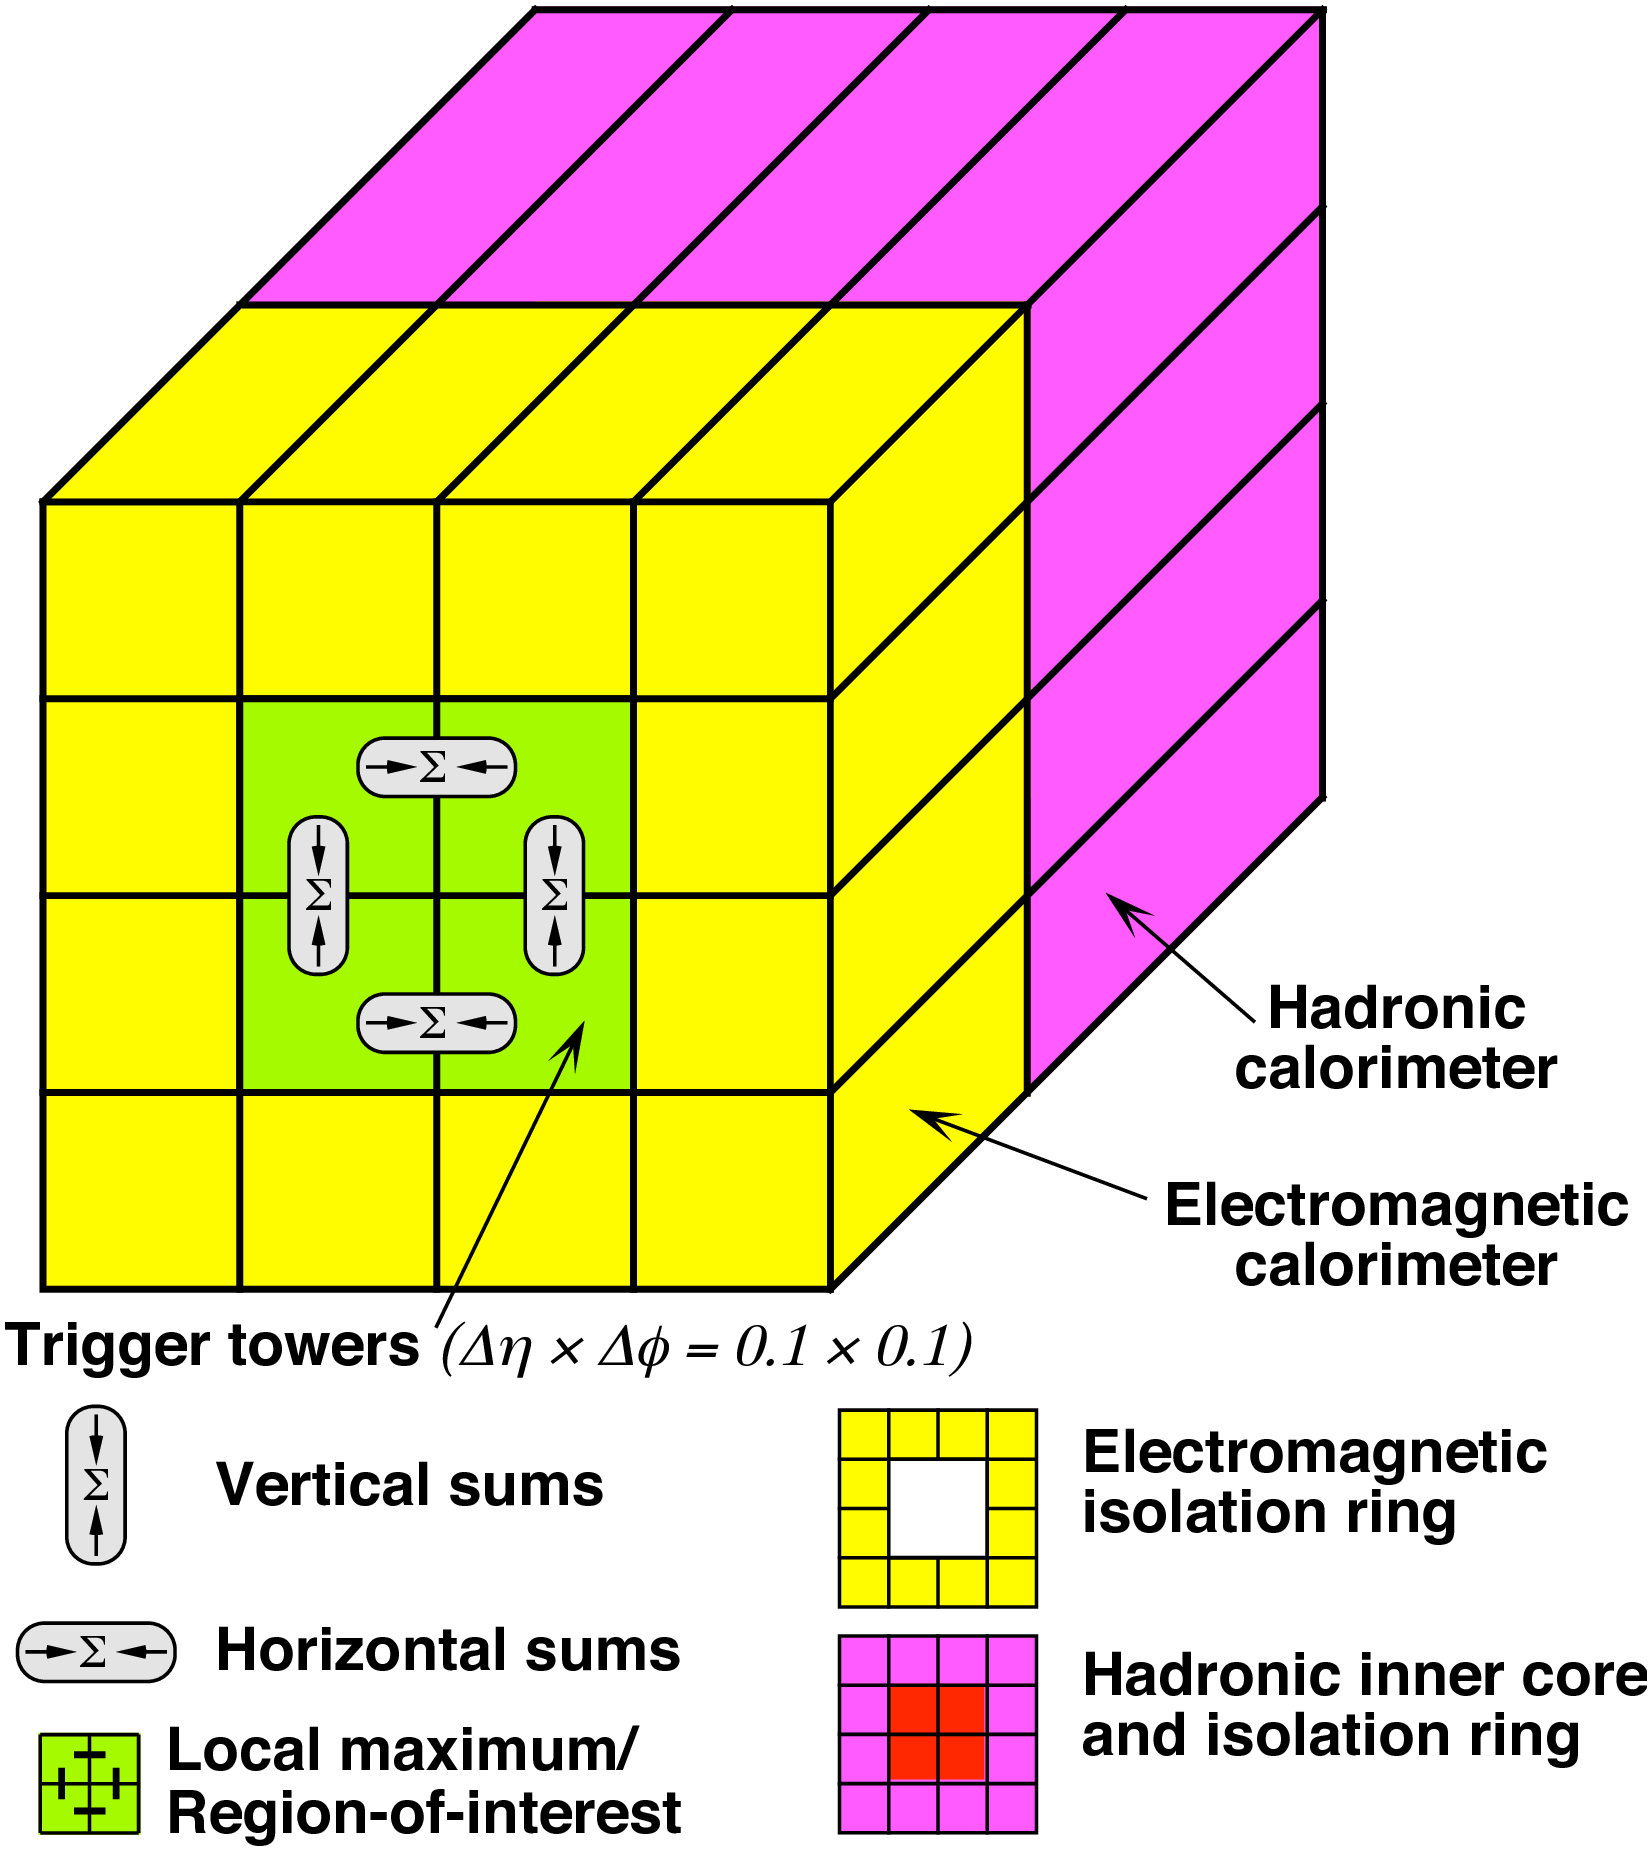
\includegraphics[width=2.5in]{figures/chapter3/l1calo.png}
    \caption{Schematic view of the trigger towers used as input to the L1 Calorimeter trigger algorithms}
    \label{fig:l1calo}
\end{figure}

The HLT is a large farm of CPUs which further analyze the ROIs defined by the L1 trigger; it has an output frequency of around 1kHz. The HLT runs multiple feature extraction algorithms on these ROIs to request event-data fragments and then performs simplified reconstruction algorithms (also referred to as online reconstruction) on these data subsets. The reconstructed features are passed to a boolean decision tree which determines if the trigger conditions are satisfied and, if so, the event data is processed through the Data Acquisition System where it is stored at the experiment site and sent through the Tier 0 computing facility (described further in Section \ref{sec:storage}) \cite{trig_2017}.\\

\subsubsection{Trigger Menus}
The full collection of all L1 and HLT triggers are referred to as the trigger menu, which allows physics analyzers to select events with desired signatures. The frequency at which a trigger flags events for storage is called the trigger rate; prescales are used in some triggers to reduce the rate of data output by randomly rejecting a defined fraction of passed events. The trigger menu is divided into several categories:
\begin{itemize}
    \item primary triggers: used for physics analyses and typically un-prescaled. These triggers cover all physics signatures relevant to ATLAS research including electrons, photons, muons, taus, jets, and missing energy.
    \item support triggers: used for efficiency and performance measurements or monitoring; typically highly prescaled.
    \item alternative triggers: used to implement new or experimental reconstruction algorithms that differ from primary or support trigger design
    \item backup triggers: have tigther selections and lower rates than primary and secondary triggers
    \item calibration triggers: used for detector calibration. They often operate at a very high rate but store small events with only the information relevant to calibration \cite{trig_2015}.
\end{itemize}
The main triggers for 2017 are shown in Table \ref{tab:trig_menu}, along with their corresponding rates. The physics trigger group rates for L1 and HLT as a function of luminosity blocks is shown in Figure \ref{fig:trig_rates}.

\begin{table}
    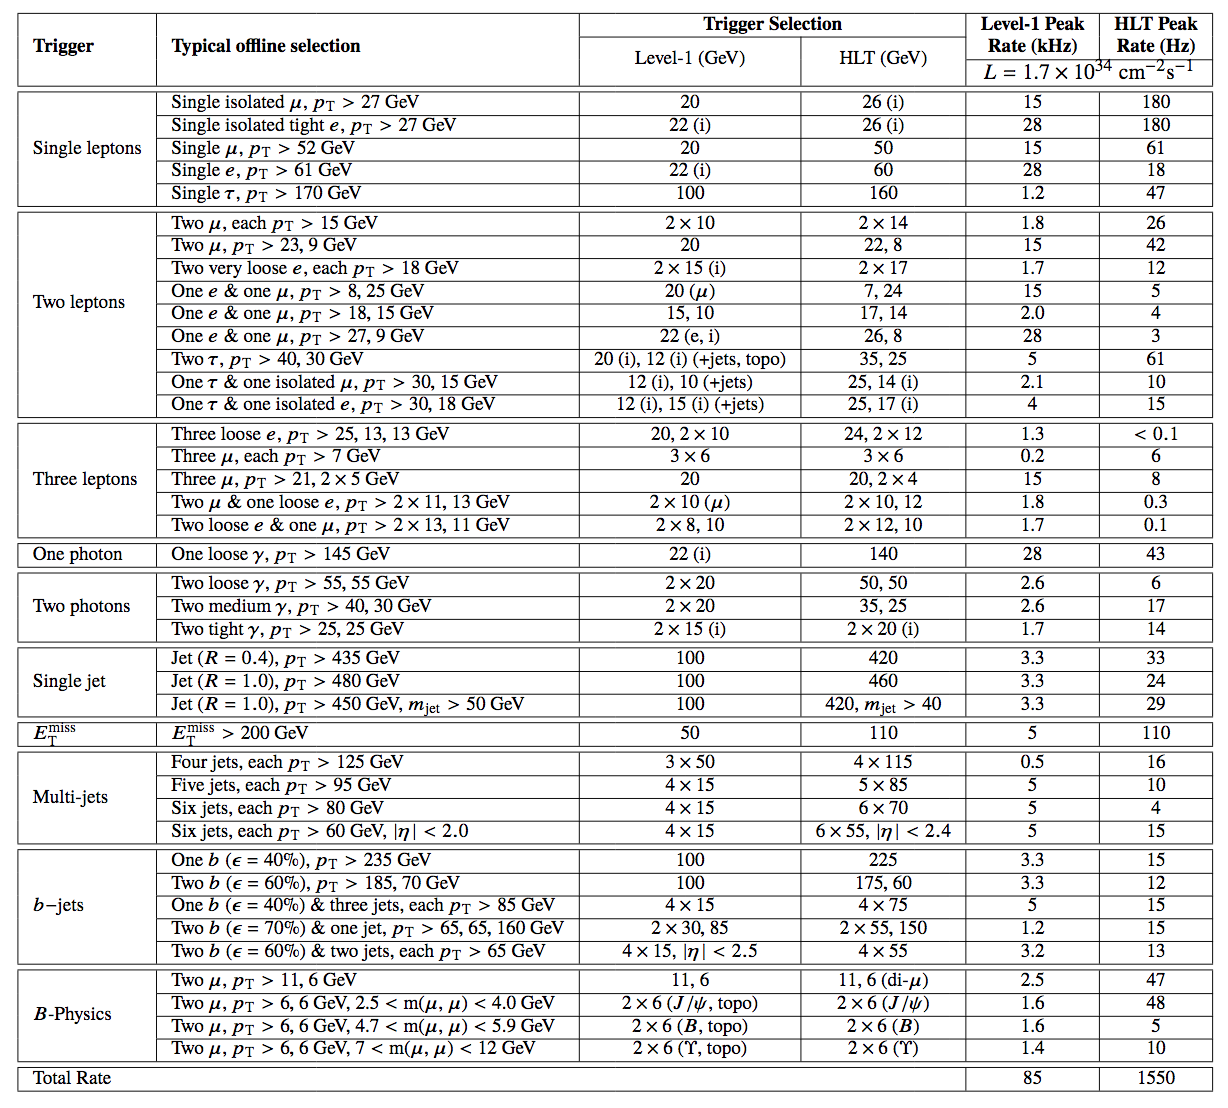
\includegraphics[width=6in]{figures/chapter3/2017_trig_menu.png}
    \caption{The main ATLAS triggers for the 2017 trigger menu with observed rates \cite{trig_2017}.}
    \label{tab:trig_menu}
\end{table}

\begin{figure}[h]
    \begin{subfigure}
        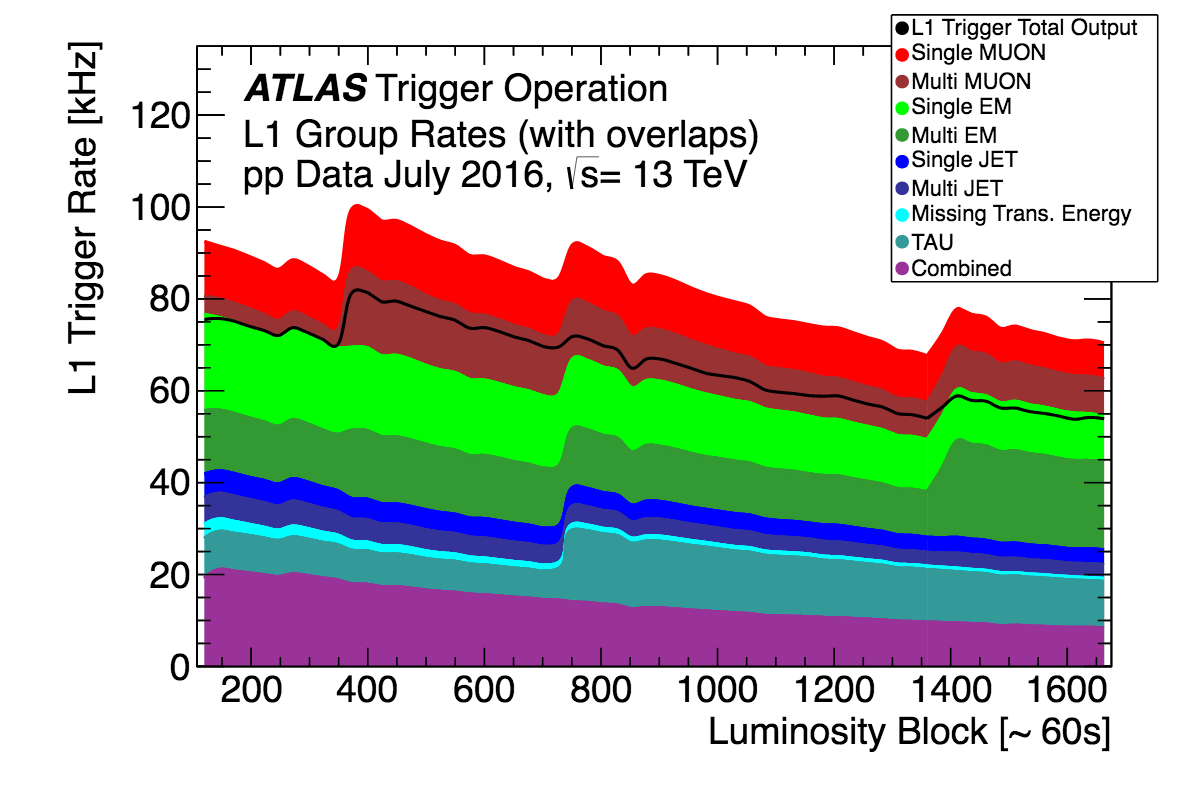
\includegraphics[width=2.5in]{figures/chapter3/l1_rates.pdf}
    \end{subfigure}
    \begin{subfigure}
        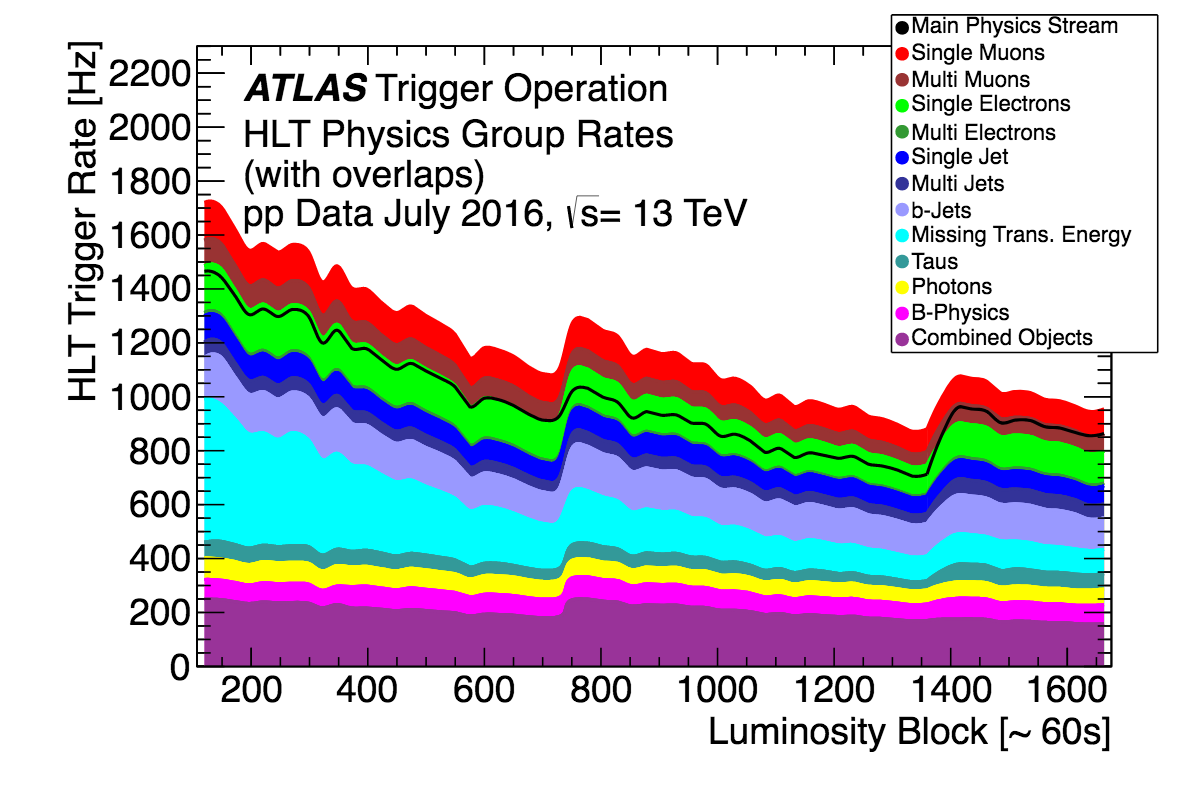
\includegraphics[width=2.5in]{figures/chapter3/hlt_rates.pdf}
    \end{subfigure}
    \caption{Physics trigger group rates for the L1 (left) and HLT (right) as a function of the number of luminosity blocks from a fill taken in July 2016 \cite{trig_pub}.}
    \label{fig:trig_rates}
\end{figure}

%%subsec: storage
\subsection{Storage}\label{sec:storage}
The Worldwide LHC Computing Grid (WLCG) provides global resources to store, distribute, process, and analyze the over 50 PB of data produced by the LHC every year \cite{wlcg_web}. WLCG is divided into 4 levels called Tiers. All data recorded by ATLAS and other LHC experiments first enters the CERN Data Center, referred to as Tier 0, where raw detector data is reconstructed into physics objects. The ATLAS algorithms run at Tier 0 are described further in Section \ref{sec:data_proc}. Tier 0 is connected by 10 GB/s optical fibers to 13 Tier 1 centers around the world. Tier 1 centers are responsible for storing raw and reconstructed data, performing large-scale data reprocessing, and storing simulated data produced at Tier 2 centers. The work described in this dissertation was primarily conducted using the BNL ATLAS Tier 1 center \cite{bnl}.\\

The 155 Tier 2 systems are typically located at universities or other scientific facilities with sufficient computing power. Tier 2s are used primarily for generation and reconstruction of simulated data. Finally, Tier 3 systems are used by individual physicists or research groups to access the WLCG and conduct individual analysis tasks \cite{grid_tdr}.\\

All ATLAS WLCG data is managed by the Rucio Distributed Data Management System \cite{rucio}. Rucio ensures that all ATLAS researchers can manage and process data in a heterogeneous distributed environment. The system manages more than 300 PB of data contained in more than 830 million files using over 130 global data centers \cite{rucio_run2}. 

%%% SEC: SIMULATION
\section{Simulation}
Simulated data is used to understand and inform detector hardware, design reconstruction and analysis software, and interpret predictions and results of various theories. The ATLAS simulation infrastructure is comprised of a range of software which generates particle collision simulations and carries them through the process of hadronization, detector interactions, and digitization. The output of the simulation chain is identical in structure to the output of the TDAQ system. The entire simulation flow is shown in Figure \ref{fig:sim_flow}. The ATLAS simulation chain relies on randomized methods of Monte Carlo sampling, and simulated data is often referred to as simply `Monte Carlo' (MC).\\ 

\begin{figure}[h]
    \centering
    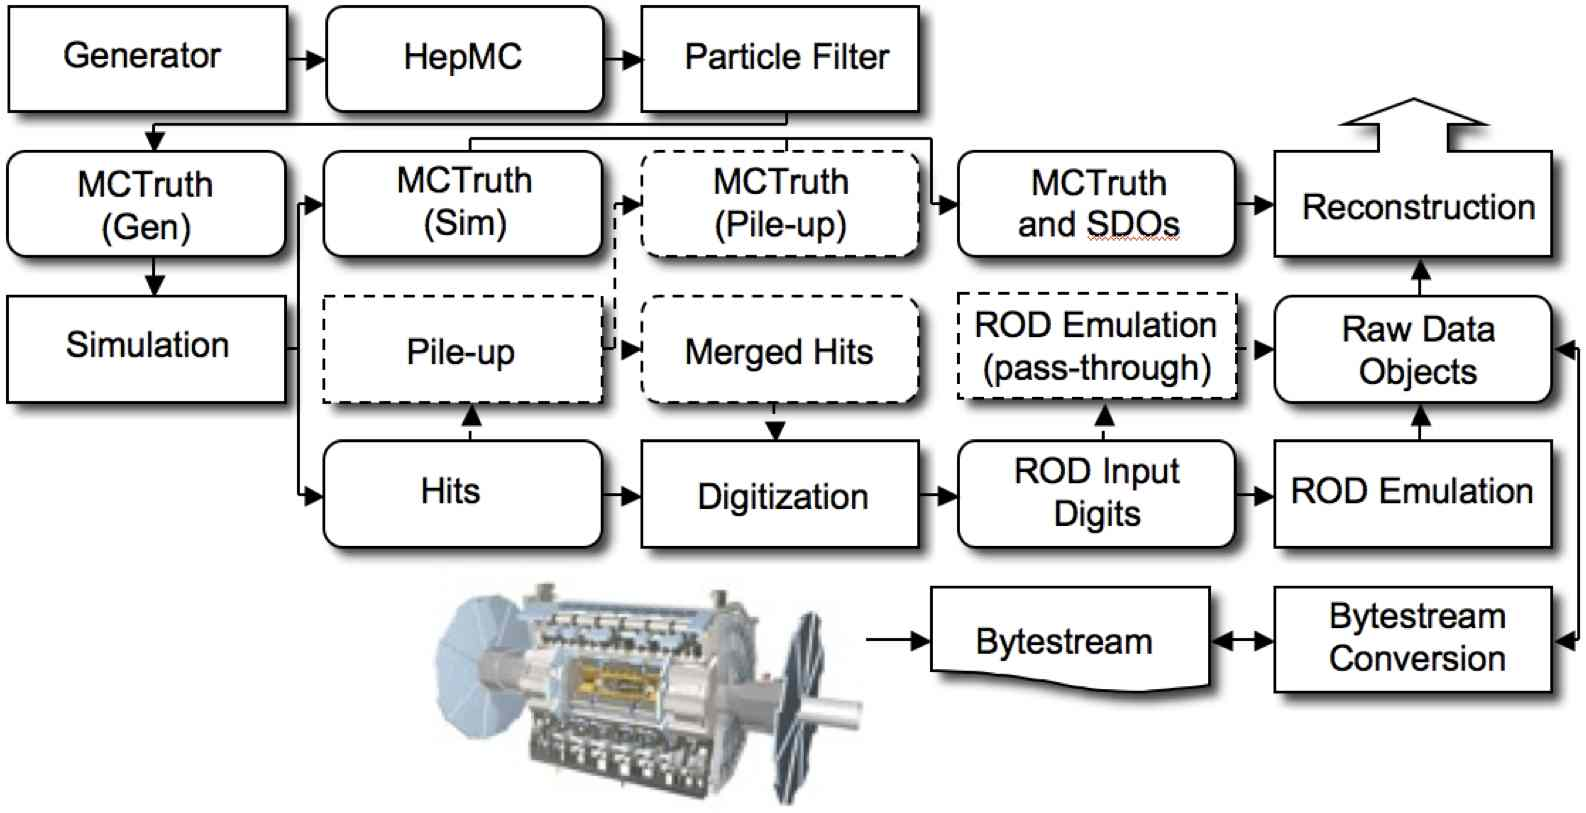
\includegraphics[width=5in]{figures/chapter3/sim_flow.png}
    \caption{The flow of the ATLAS simulation software, from event generators (top left) through reconstruction (top right). Algorithms are placed in square-cornered boxes and persistent data objects are placed in rounded boxes. The optional pile-up portion of the chain, used only when events are overlaid, is dashed \cite{sim_paper}.} 
    \label{fig:sim_flow}
\end{figure}

%%subsec: event gen
\subsection{Event Generation}
Physics generators that simulate the desired hard-scattering processes and subsequent decays are the first stage of MC simulation. These generators produce a list of particles created by proton-proton collisions that are expected to exist long enough to propagate through the detector. The generators also record ``truth" information listing every incoming and outgoing particle regardless of whether it is passed to the later simulation stages \cite{sim_paper}.\\

ATLAS simulation utilizes several externally supported general purpose MC generators which employ similar computation strategies. The first step is generating the central hard-scattering process. This relies on matrix-element based computations and these matrix-elements can be hard coded by the developer or calculated to a certain order in perturbation theory by the generator. The evolution of the produced particles due to QCD (Chapter 1) is then described by parton showering which connects the hard scale of colored parton creation to the hadronization scale. At the hadronization scale, on the order of a few $\Lambda_{QCD}$, QCD partons are transformed into primary hadrons by applying phenomenological fragmentation models based on effective field theories. Generators also account for QED bremsstrahlung radiation and potential secondary hard or semi-hard interactions of remaining hadron remnants. The combination of these event generation stages is represented pictorially for a single ttH event in Figure \ref{fig:event_gen} \cite{sherpa_egen}.\\

General purpose generators that function as described above include Pythia \cite{pythia}, Herwig \cite{herwig}, MadGraph \cite{madgraph}, and Sherpa \cite{sherpa_egen}. These generators are typically FORTRAN or C++ based and their outputs are all translated into the standard HepMC event record format \cite{hepmc}. The analyses presented in this dissertation primarily utilize Pythia and Sherpa generated MC samples. These general purpose generators described above are often interfaced with specialized generators to improve the description of certain final states. These include Tauola for tau lepton decays \cite{tauola}, EvtGen for B meson and hadron decays \cite{evtgen}, Alpgen for hadronization in final states with multiple well-separated jets \cite{alpgen}, MC@NLO for top events \cite{mcnlo}, and AcerMC for W and Z decays with several jets \cite{acermc}.\\

\begin{figure}[h]
    \centering
    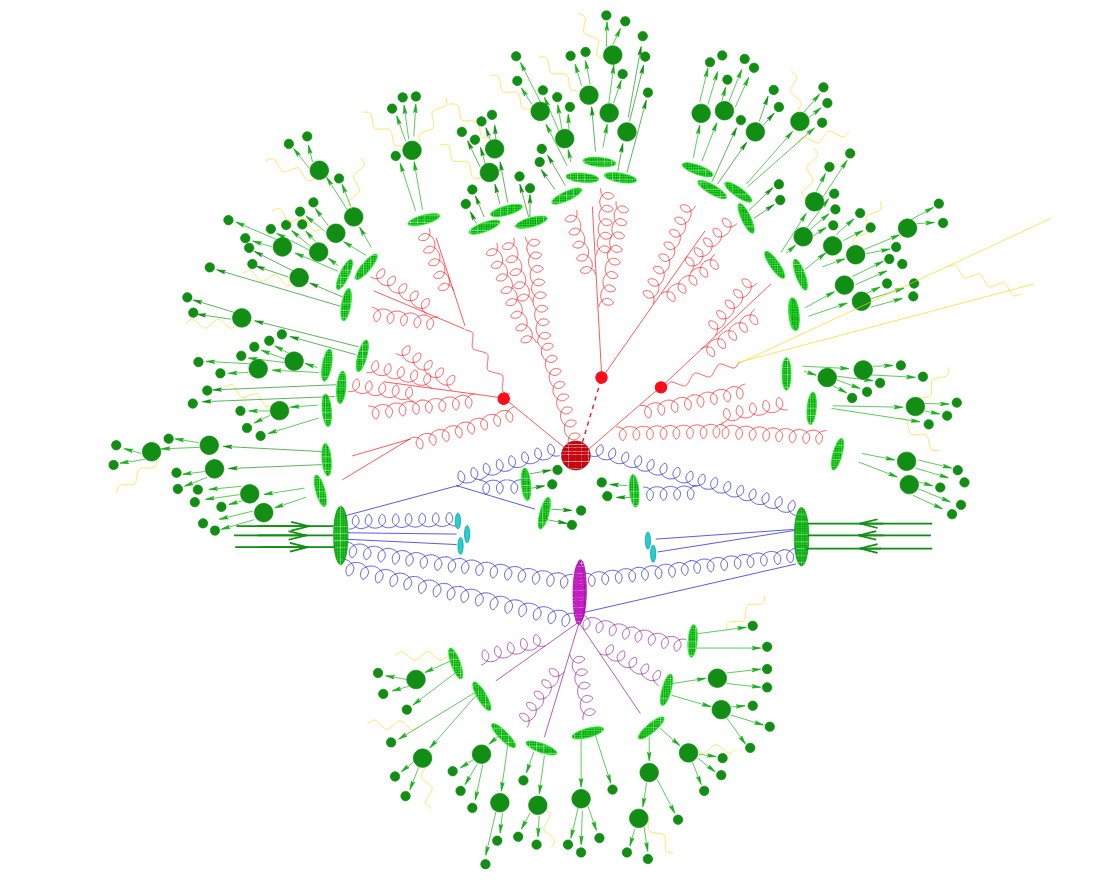
\includegraphics[width=5in]{figures/chapter3/event_gen.png}
    \caption{Pictorial representation of a generated ttH event. The central hard interaction is shown as the central red circle, which is followed by the subsequent decays of the Higgs and top quarks (smaller red circles). Additional hard radiation due to QCD is produced (blue) as well as a secondary hard interaction (purple). Finally, hadronization (light green) and hadron decay (dark green) occurs. Photon radiation is represented in yellow and occurs at multiple stages \cite{sherpa_egen}.}
    \label{fig:event_gen}
\end{figure}

%%subsec: detector sim
\subsection{Detector Simulation}
The particle lists created by event generators are further processed through a detector simulation which describes how the particles interact with various physical components of the ATLAS detector and how those interactions are read out by detector electronics.\\

The ATLAS Simulation group supports a centralized simulated detector geometry written in GEANT4 \cite{geant4}, a widely used scientific simulation toolkit. The ATLAS detector description contains nearly 5 million volumes comprised of over 300 different materials. A summary of these volumes is shown in Table \ref{tab:detec_geo}. The detector simulation is revised as updates are made to the detector or when additional simulation functionality becomes available \cite{atlas_sim}.\\

\begin{table}
    \centering
    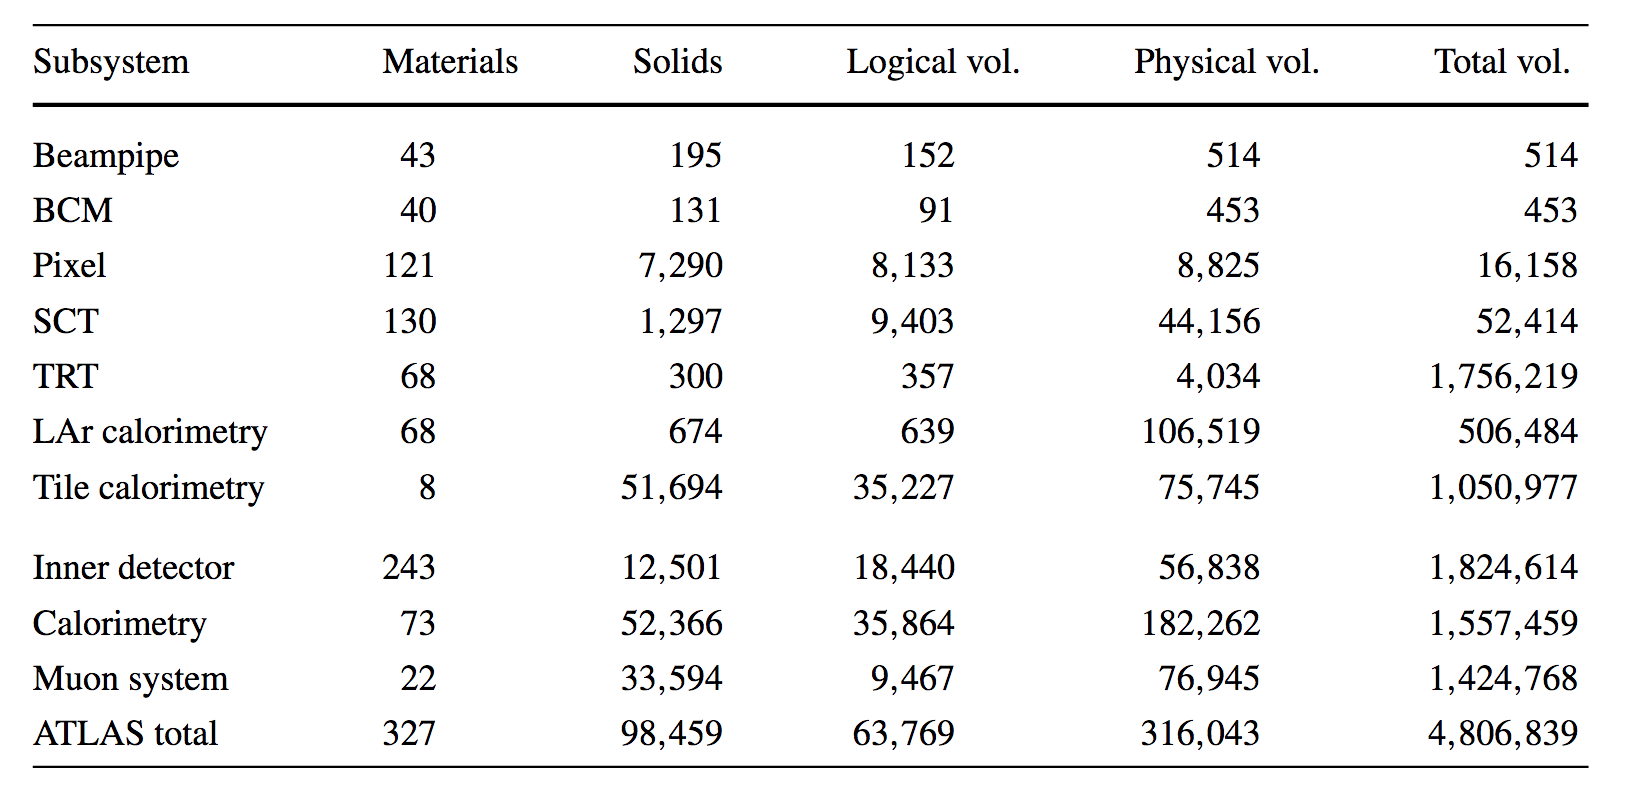
\includegraphics[width=5in]{figures/chapter3/detec_geo.png}
    \caption{Numbers of materials and volumes used to construct the ATLAS detector simulated geometry \cite{sim_paper}.}
    \label{tab:detec_geo}
\end{table}

GEANT4 also provides physics models to simulate different processes of particle interaction with materials including the photoelectric effect, Compton scattering, bremsstrahlung, ionization, multiple scattering, decays, nuclear interactions and more. These physics models rely on iterative Monte Carlo sampling. The models are applied as appropriate to generated particles traveling through the simulated detector geometry. Truth information, taken from the event generation record, including real tracks and decays of particles is also stored.\\

The final simulation step is digitization, which transforms the hits and energy deposits created by the detector simulation into Raw Data Objects identical in structure to the electronic readouts of the physical detector. Pileup overlay, detector noise, and other backgrounds such as cosmic ray muons are also added to the simulation during digitization. Truth information from the digitization stage is stored as Simulated Data Objects (SDOs) which act as maps from generated truth particles to simulated detector readouts. SDOs can be used later to validate reconstruction algorithms and quantify their performance \cite{sim_paper}.\\

The full simulation chain described above is incredibly time and CPU intensive and as such is not possible to provide complete simulations with high statistics for all relevant physics studies. A variety of programs, collectively referred to as Fast Simulations, exist to complement the full simulation in cases when full accuracy isn't necessary. Approximately 75\% of full simulation time is spent simulating electromagnetic particles; the Fast G4 Simulation expedites this process by replacing low energy electromagnetic particles with pre-simulated showers \cite{g4_sim}. The ATLFAST-II package provides large simulation statistics by directly simulating the input to reconstruction algorithms rather than separate detector geometry and digitization steps. It contains two modules: FATRAS \cite{fatras}, which speeds up Inner Detector and Muon Spectrometer simulations by generating only the track input required by reconstruction algorithms, and FastCaloSim \cite{fastcalo}, which reduces particle-calorimeter interaction simulation time by directly calculating the energy of single particle showers. 

%% SEC: PROCESSING
\section{Data Processing}\label{sec:data_proc}
Both recorded and simulated data are processed through the ATLAS reconstruction and object identification chain before being used in physics analyses. Reconstruction algorithms are typically detector-component specific and, when combined, create particle candidates. Identification algorithms specific to individual SM particles are supported by dedicated Working Groups within the collaboration and further classify particle candidates. Datasets with labeled particles, trigger history, and in the case of MC, truth information, are then used by individual researchers for physics analyses.

%%subsec: recon
\subsection{Reconstruction}
The particle identification algorithms described in Section \ref{sec:id} typically take partially reconstructed objects as inputs, rather than directly using detector read-out information. These reconstructed objects take the form of tracks left in the Inner Detector, interaction vertices, energy deposit clusters in the calorimeters, or matched combinations of these. The common algorithms used to reconstruct these objects are described below. 

\subsubsection{Tracking}\label{sec:tracking}
The path a particle takes through the inner detector is called a track, and track finding algorithms seek to reconstruct these paths by connecting hits in various layers of the inner detector. These algorithms must provide parameters to fully describe the track (impact parameters $d_0$ and $z_0$, angles $\phi$ and $\theta$, and particle charge and momentum) and account for various particle-material interactions such as scattering, ionization loss, bremsstrahlung, and hadronization. The full track finding process proceeds in several steps \cite{track_run1}.\\

First, a connected component analysis is used to cluster pixels and strips in a given detector component together. These clusters are formed when when the combined deposited energy in cells sharing an edge or corner exceeds a certain tunable threshold. These clusters are then transformed into 3-D objects called space-points; in the pixel detector one cluster becomes one spacepoint while in the SCT clusters from both sides of a strip are required \cite{track_run2}. Spacepoints can be classified as single-particle (all energy comes from a single particle) or merged (multiple particles deposit energy in the same cells) as shown in Figure \ref{fig:track_clus}.\\

\begin{figure}[h]
    \begin{subfigure}
        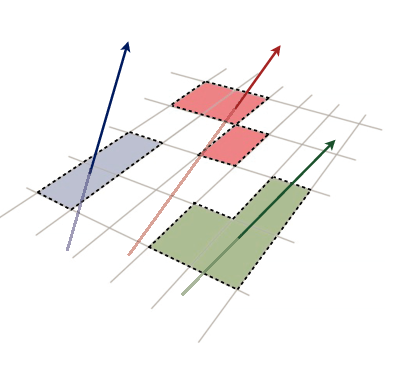
\includegraphics[width=2.5in]{figures/chapter3/single_track_clus.png}
    \end{subfigure}
    \begin{subfigure}
        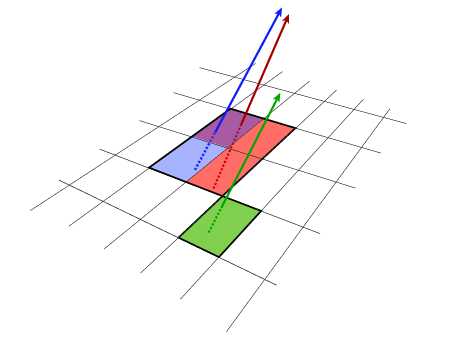
\includegraphics[width=2.5in]{figures/chapter3/merged_track_clus.png}
    \end{subfigure}
    \caption{Illustraion of a single particle space-point (left) and merged particle space-point (right) on a pixel sensor \cite{track_run2}.}
    \label{fig:track_clus}
\end{figure}

Space-points are then combined in sets of three, called track seeds, which serve as the basis for track candidates. Track seeding allows full track finding algorithms to consider a large number of possible tracks while still providing an initial momentum estimate. The quality of final tracks depends on which sub-detector the track seed originates in, so seeds are ordered to prioritize SCT-only, then pixel-only, then mixed-detector seeds. The track seeds are then passed to a combinatorial Kalman filter \cite{kalman} which builds full track candidates by adding additional compatible space-points from remaining layers of the inner detector.\\

An ambiguity solver algorithm is used to process cases where multiple track candidates share the same space point. Tracks are scored by considering track momentum, track holes, track fit accuracy, and assigned space-points. Tracks are then processed in descending order of score and shared space-points are either assigned as uniquely corresponding to that track or merged with another track, the space-point is removed from the track, or the track is rejected entirely. Track candidates which pass the ambiguity solver are assigned a final neural network calculated parameterized fit using all available track information \cite{track_run2}. Neural networks are described further in Chapter 4.\\

Additional TRT-based track seeding is used in certain ROIs corresponding to electromagnetic calorimeter clusters created by converted photons \cite{tracking_improvements}. Muon specific reconstruction and identificiation algorithms also utilize track fitting in the Muon Spectrometer, and this is described further in Section \ref{sec:muons}.\\

ATLAS track reconstruction is highly efficient as shown in Figure \ref{fig:track_eff}. However, the detector resolution limits the performance potential of current techniques in high pile-up environments. Revising the ATLAS tracking software, potentially by incorporating additional ML techniques, is an on-going research area for the HL-LHC.

\begin{figure}[h]
    \centering
    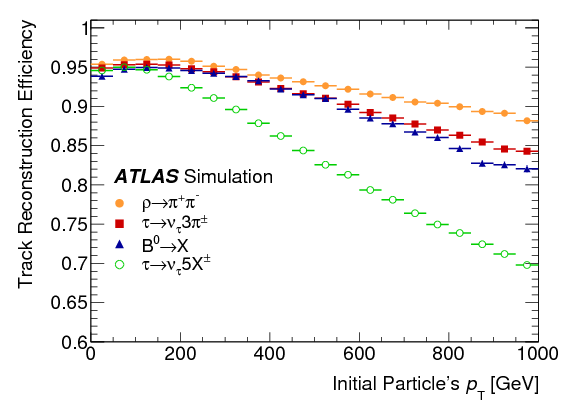
\includegraphics[width=4in]{figures/chapter3/track_eff.png}
    \caption{Single track reconstruction efficiency as a function of particle $p_T$ for a $\rho$ (orange), three prong $\tau$ (red), five prong $\tau$ (green), and $B^0$ (blue) \cite{track_run2}.}
    \label{fig:track_eff}
\end{figure}

\subsubsection{Vertexing}
The points where multiple tracks intersect are called vertices. Vertices are found using an iterative algorithm which seeds vertices using the z-position at the beamline of the reconstructed tracks by applying a $\chi^2$ fit to the seed and nearby tracks. Tracks originating more that 7$\sigma$ away from the vertex are used to seed a new vertex and this process is repreated until all possible vertices are defined. All vertices are required to have at least two associated tracks. Vertices are associated with interactions by calculating the sum of the squares of $p_T$ of associated tracks, and at least 50\% of the energy of an interaction must be accounted for by the assigned tracks. This ensures that final vertex position is influenced most heavily by tracks of particles coming from that interaction. The vertex with the highest $(p_T)^2$ sum is called the primary vertex.\cite{vertex}\\ 

A new vertexing algorithm is being developed based on image processing ML techniques. This algorithm simultaneously identifies all potential vertices in a given event using plots of the identified tracks as input. This algorithm is more robust to pile-up and reduces the CPU time required for vertexing, both of which are important considerations for HL-LHC algorithm design \cite{tracking_improvements}.\\

The vertex reconstruction efficiency for 2018 is shown in Figure \ref{fig:vertex} by comparing the average number of reconstructed vertices to the average number of interactions per bunch crossing ($\mu$). The efficiency decreases with increasing $\mu$ due to shadowing, where two or more interactions are too close in proximity to be resolved individually.

\begin{figure}[h]
    \centering
    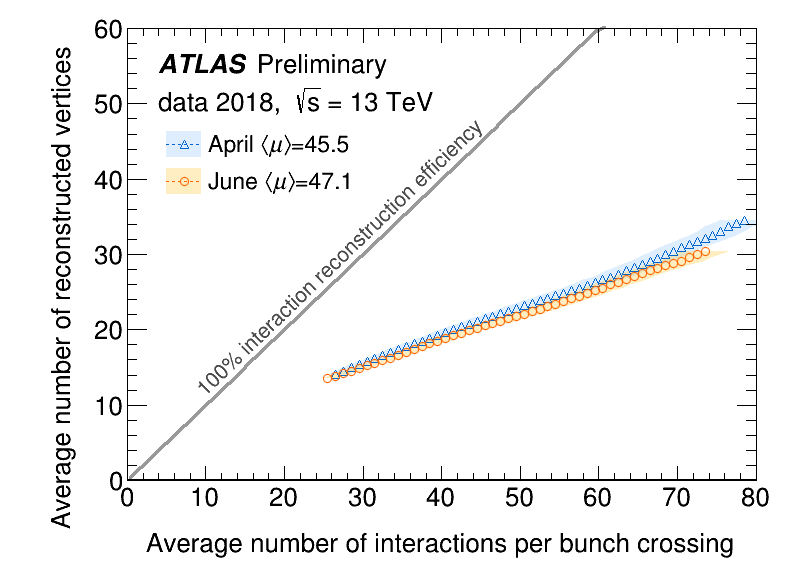
\includegraphics[width=4in]{figures/chapter3/vertex_eff.png}
    \caption{The number of vertices reconstructed as a function of the average interactions per bunch crossing for two fills taken in 2018 \cite{vertex_pub}.}
    \label{fig:vertex}
\end{figure}

\subsubsection{Calorimeter Clustering}\label{sec:clustering}
Particles deposit energy in a spread of calorimeter cells both laterally and longitudinally. Dedicated algorithms group the cells corresponding to an individual particle together and assign a cumulative energy value to the constructed cluster. ATLAS uses two types of clustering algorithms which are described below.\\

The ``sliding window" clustering algorithm sums cells within a fixed-size section of the calorimeter. This algorithm proceeds in three steps. First, the calorimeters are divided into a grid of sections of size $\Delta\eta\times\Delta\phi$, called towers, and the energy of all cells in all layers within the tower is summed. Then a window of fixed-size $N_{\eta}^{window}\times N_{\phi}^{window}$ is moved across the grid of towers and when the energy contained within the window is a local maximum and exceeds a preset threshold, the group of towers within the window is categorized as a precluster. The location of the precluster is set as the energy-weighted center of all cells within a separate fixed-size window positioned on the tower at the center of the sliding window. The final cluster is formed by adding all additional cells within an $N_{\eta}^{cluster}\times N_{\phi}^{cluster}$ window of the seed position.\\ 

Sliding window clustering is used to form the clusters used in the  electron, photon, tau, and jet identification algorithms. The sliding window, position window, cluster, and tower sizes, as well the energy threshold can be adjusted to form separate input clusters for these different objects \cite{calo_clustering}.\\

 Topological clustering is an alternative algorithm which iteratively adds neighboring cells to an initial seed cluster when the energy in the new cell is above an expected noise threshold. This method results in final clusters of varying size, in contrast to the sliding window algorithm. All cells with a signal-to-noise above an initial threshold (related to the expected electronics noise from gain and detector conditions) are identified as cluster seeds. The seeds are sorted in descending order of signal strength, and all neighboring cells are considered for addition to the cluster. A neighboring cell is added if it has not already been used as a seed and its signal-to-noise ratio is above the set neighbor threshold. If a cell is adjacent to more than one seed, the two seeds are merged. An example of a topologically clustered jet event is shown in Figure \ref{fig:topo}.\\

\begin{figure}[h]
    \centering
    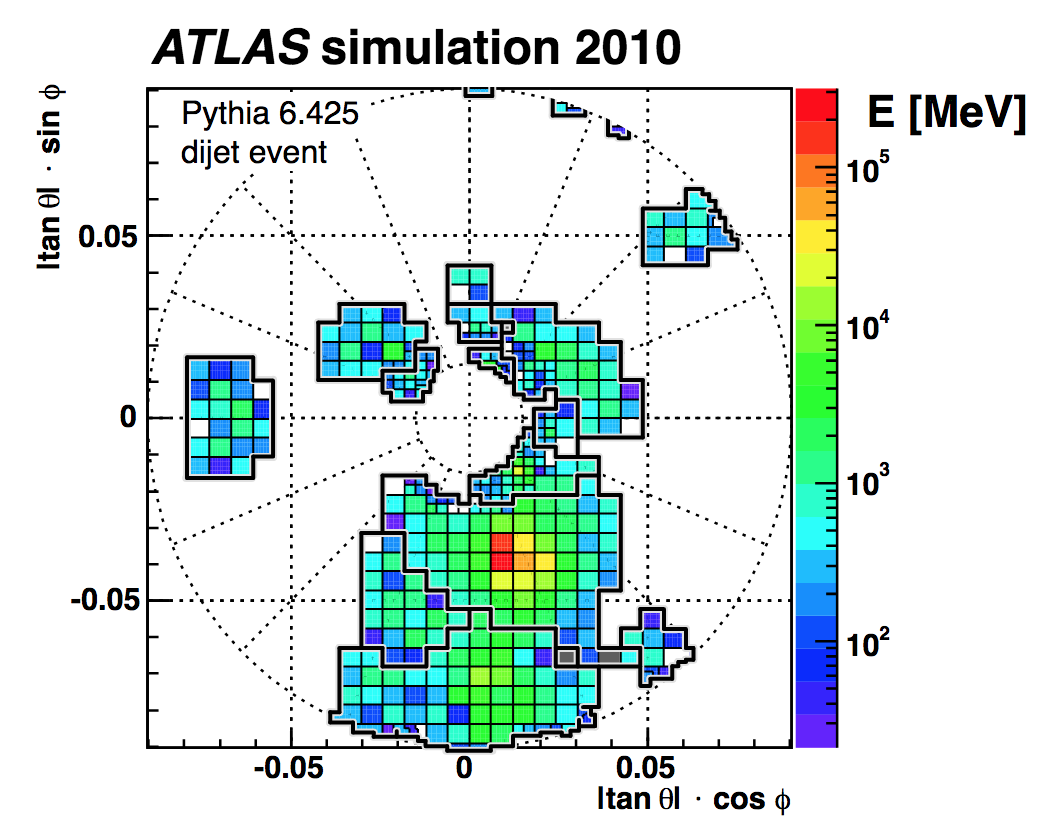
\includegraphics[width=4in]{figures/chapter3/topo_clust.png}
    \caption{Clusters for a simulated dijet event created in the FCAL using the topological clustering algorithm \cite{topo_clustering}.}
    \label{fig:topo}
\end{figure}

Topological clustering is very effective at suppressing noise in large clusters, and thus is used for jet and missing energy algorithms. The signal-to-noise thresholds for seeding and adding neighbors can be adjusted for different applications, as can the number of neighboring cells considered. Additional details can be found in \cite{topo_clustering}.\\

The final energy assigned to the constructed cluster depends on the clustering algorithm used and the type of object the cluster is eventually assigned to. The callibration methods are described in detail in \cite{egam_calib} for electrons and photons and in \cite{had_calib} for taus and jets.\\

%%subsec: ID
\subsection{Identification}\label{sec:id}
The individual algorithms used to fully reconstruct and identify the objects relevant to the $VH,H\rightarrow\tau\tau$ analysis described in Chapters 6 and 7 are outlined below. The software used for identifying electrons is described in detail in Chapter 5. 

%% muons
\subsubsection{Muons}\label{sec:muons}
Accurately reconstructing and identifying muons is essential to a variety of ATLAS analyses including the Higgs boson discovery \cite{higgs_paper} and subsequent measurements, other SM measurements (eg \cite{zz_paper}), and BSM searches (\cite{muon_bsm} and many others). The dedicated muon algorithms must work for a variety of muons ranging from soft, non-isolated muons produced in jets to high $p_T$ muons from W/Z decays or new physics. The algorithms described below make use of all components of the ATLAS detector: tracks in the Inner Detector, track stubs in the Muon Spectrometer, and energy deposits in the calorimeters and Muon Spectrometer.\\

In addition to Inner Detector tracks, which are constructed as described in Section \ref{sec:tracking}, muon algorithms also make use of tracks in the Muon Spectrometer (MS). Tracks are first reconstructed in individual components of the MS using a Hough transform in the MDT segments and associated trigger chambers and a combinatorial search in the CSC. Full track candidates are then formed by matching segments in different layers of the MS using a segment-seeded combinatorial search that begins with seeds in the middle MS layers. Finally, track candidates are fit using a global $\chi^2$ fit \cite{muons_run2}.\\

The MS-track candidates are then combined with Inner Detector tracks and calorimeter clusters to form four types of muon candidates (demonstrated graphically in Figure \ref{fig:muon_types}):
\begin{itemize}
    \item Combined muons: tracks in the MS and Inner Detector are combined using a global refit. The $VH,H\rightarrow \tau\tau$ analysis described in this dissertation uses only combined muons.
    \item Segment-tagged muons: tracks in the Inner Detector are classified as muon candidates if they can be extrapolated and matched to at least one track segment in the MS.
    \item Calorimeter-tagged muons: tracks in the Inner Detector are classified as muon candidates if they can be matched to a calorimeter cluster consistent with a minimum-ionizing particle.
    \item Extrapolated or stand-alone muons: a track in the MS is extrapolated to the Inner Detector.
\end{itemize}

\begin{figure}[htb!]
    \centering
    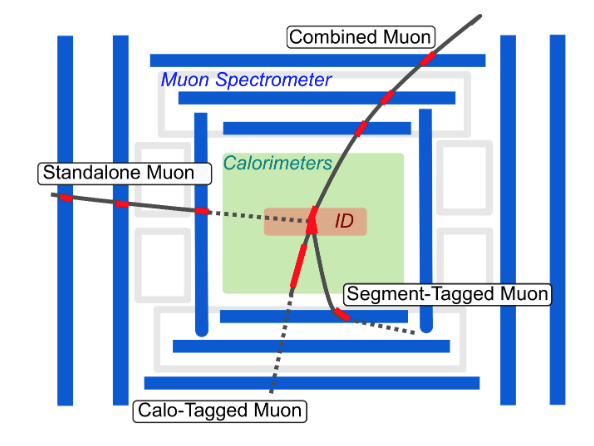
\includegraphics[width=3.5in]{figures/chapter3/muon_types.png}
    \caption{Depiction of the four types of reconstructed muons}
    \label{fig:muon_types}
\end{figure}

Overlap between the muon types is resolved in the order they are listed above \cite{muons_run2}. An example of muon reconstruction efficiency is shown in Figure \ref{fig:muon_reco}.

\begin{figure}[htb!]
    \centering
    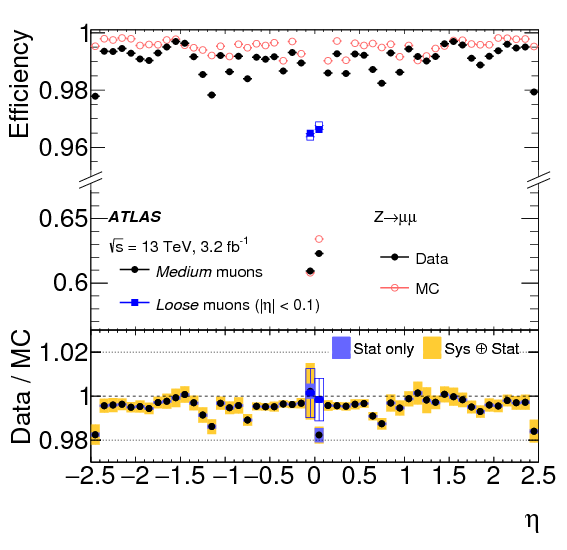
\includegraphics[width=4.5in]{figures/chapter3/muon_reco_perf.png}
    \caption{Muon reconstruction efficiency as a function of $\eta$ measured in $Z\rightarrow \mu\mu$ events for muons with $p_T>$10 GeV \cite{muons_run2}.}
    \label{fig:muon_reco}
\end{figure}

Muon candidates are then officially identified as muons by placing requirements on fit quality and momentum reconstruction (further described in \cite{muons_run2}). The muon Working Group in ATLAS supports four muon identification (ID) working points (Loose, Medium, Tight, and High $p_T$) to suit the efficiency and purity needs of different analyses. The efficiencies of the various operating points for muons originating in W decays is shown in Table \ref{tab:muon_id_eff}.\\

\begin{table}[htb!]
    \centering
    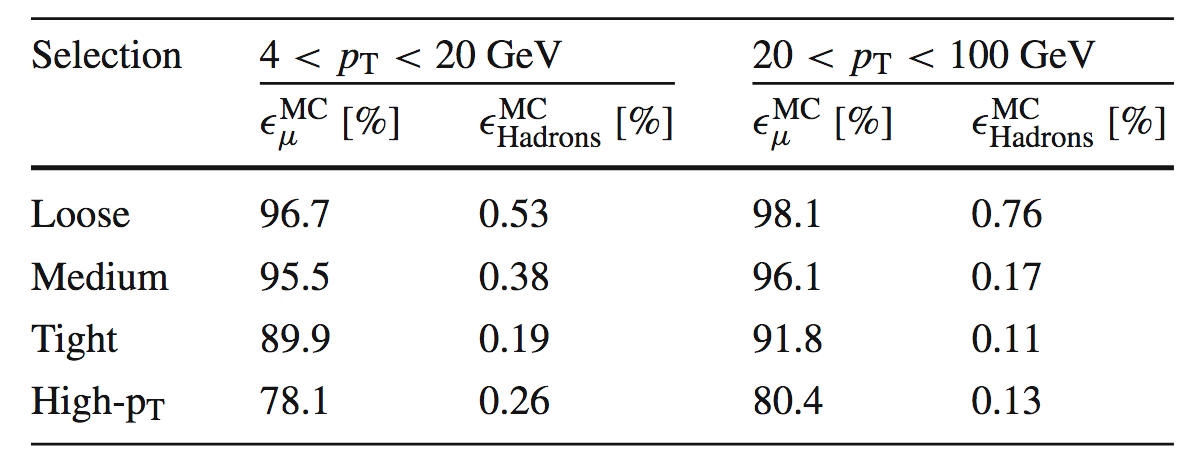
\includegraphics[width=4in]{figures/chapter3/muon_id_eff.png}
    \caption{ID efficiencies for prompt muons from W decays and the misidentification rates for hadron decays computed from a $t\bar{t}$ MC sample \cite{muons_run2}.}
    \label{tab:muon_id_eff}
\end{table}

%% jets
\subsubsection{Jets}
Jets are hadronic showers of particles that originate from some initial parton splitting. Jets are therefore not well-defined particles like electrons or muons. The goal of jet reconstruction algorithms is to group related energy deposits into a single collection and assign an accurate energy to the constructed collection.\\

Many algorithms exist to group related phase-space objects, however many of these techniques are not well suited to the specific problem of jet clustering. This is because jet clustering algorithms in ATLAS must satisfy two physics derived properties in order for the reconstructed jets to be usable in final physics analyses. These properties are Infared (IR) Safety, which means the calibrated energy of the constructed jet must be invariant to the addition of infinitely soft radiation, and Collinear Safety, which means jet properties must remain identical if a single parton is substituted for two or more collinear partons with identical momentum. Collectively, these requirements are referred to as IRC safety.\\

There are two primary classes of jet algorithms utilized by ATLAS,  both of which take topoclusters (Section \ref{sec:clustering}) as inputs. Sequential clustering algorithms group topoclusters together using two distance metrics: $d_{ij}=min(p_{ti}^ap_{tj}^a)\times\frac{R_{ij}^2}{R}$ where $a$ is an algorithm-dependent constant, $R_{ij}$ is the $\eta\text{-}\phi$ distance between the two clusters, and R is a set maximum radius for the reconstructed jets, and $d_{iB}=p_{ti}^a$, the momentum-space distance between the beam axis and the new cluster. The algorithms create an ordered list of $d_{ij}$ and $d_{iB}$ and add clusters $j$ to jet $i$ until $d_{iB}$ is the minimum in the list. There are three main sequential clustering algorithms which differ primarily on the choice of exponent $a$, and thus the distance metric. The $k_T$ algorithm has $a=2$, which allows low $p_T$ clusters to dominate, the $anti-k_T$ algorithm has $a=-2$, which allows high $p_T$ clusters to dominate, and the Cambridge/Aachen algorithm has $a=0$, removing momentum dependence from the distance metric entirely \cite{jet_algs}.\\

The second class of clustering algorithms is cone algorithms, which, as the name suggests, are based on the assumption that the particles in a jet will manifest in conical regions and thus group clusters in strict circular regions in $\eta\text{-}\phi$ space. SIScone is the only IRC safe cone algorithm, and is described in detail in \cite{jet_algs}. Figure \ref{fig:jet_algs} compares the four main jet clustering algorithms when applied to the same event with the same maximum radius $R$; the shapes, sizes, and numbers of jets change with each algorithm.\\

\begin{figure}[h]
    \centering
    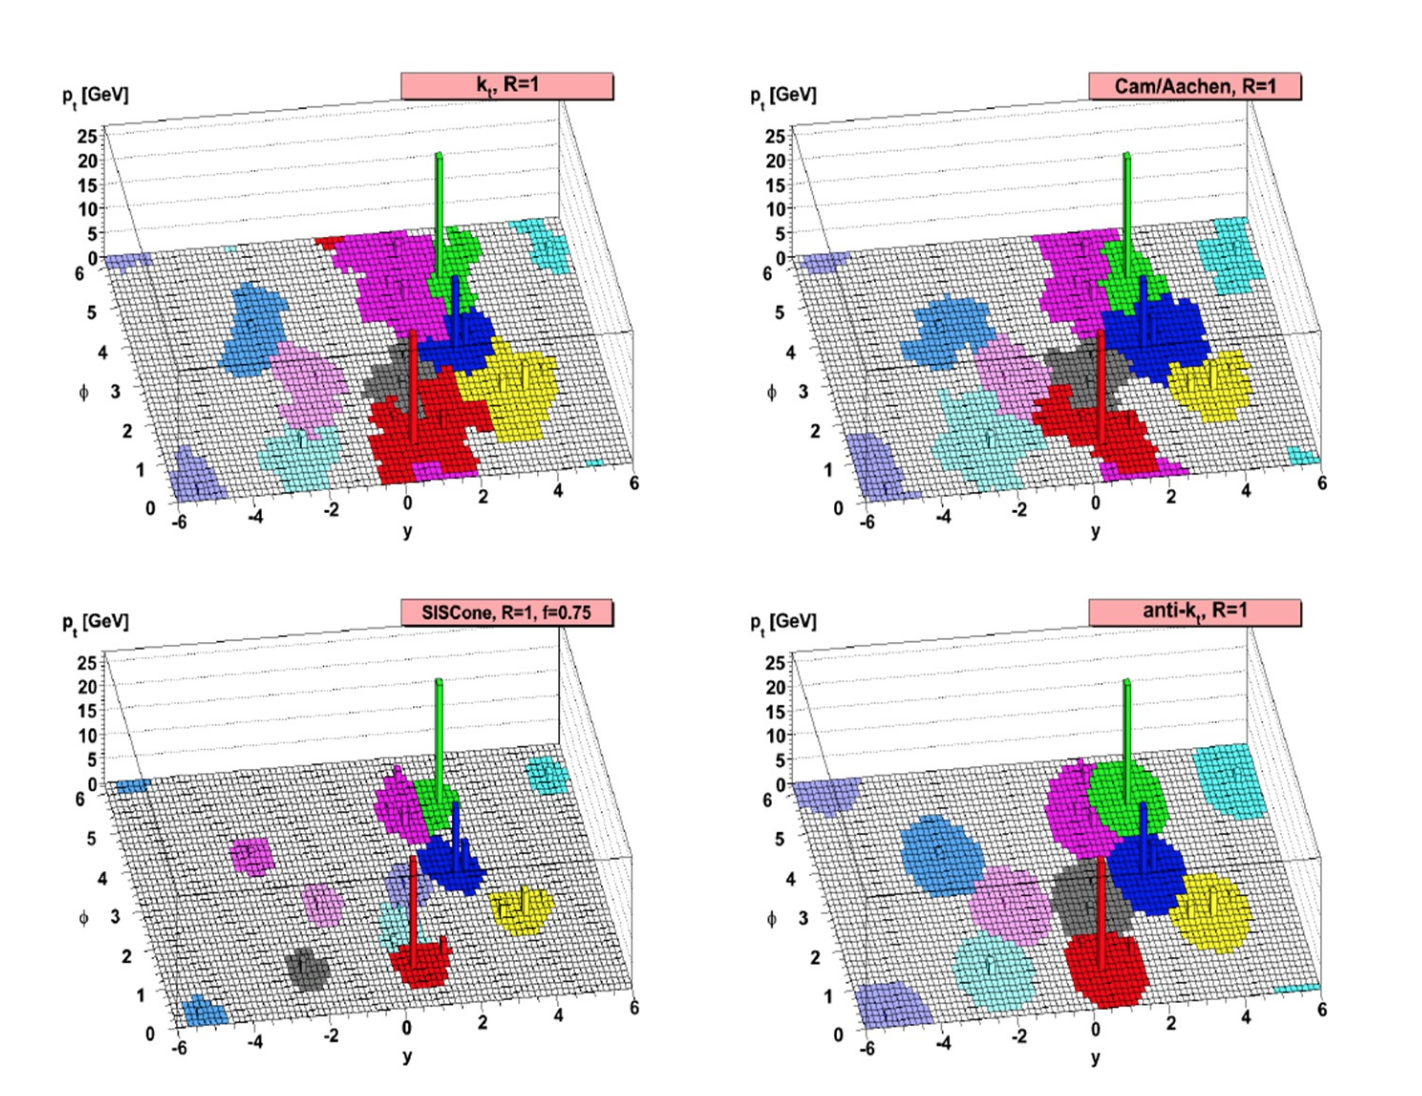
\includegraphics[width=5in]{figures/chapter3/jet_algs.png}
    \caption{The four main jet clustering algorithms performed on the same data with the same input radius \cite{jet_algs}.}
    \label{fig:jet_algs}
\end{figure}

After clustering, jets may undergo additional corrections. To mitigate pile-up effects on momentum calculations, all jets are corrected by a standard $p_T$ offset, determined in MC as a function of primary vertices, and an additional jet-area based correction. Additionally, all jets undergo energy and pseudorapidity calibration based on the relation of reconstructed to truth jets in MC samples. Jets may also undergo pruning, which removes sub-jets which contribute only a small fraction of energy, origin correction, and pile-up track subtraction \cite{jet_et_paper}.\\

After clustering and corrections, jets can be processed by a variety of tagging algorithms that exploit jet-substructure information and other kinematic variables to determine the likely initial particle causing the hadronization. These algorithms are described, for example, in \cite{b_tagging} for b-jets and \cite{w_top_tagging} for top quarks and W bosons. There is substantial recent work regarding novel, ML based jet representation and tagging methods, which is discussed further in Chapter 4.\\

%%taus
\subsubsection{Tau Leptons}
Tau leptons are produced in a range of physics processes, and in particular are of central importance to the $VH,H\rightarrow\tau\tau$ analysis presented in Chapters 6 and 7. In contrast to electrons and muons, taus have a relatively large mass (1.77 GeV) and a proper decay length of only 87 $\mu$m. Taus can decay leptonically ($\tau\rightarrow l\nu_l\nu_{\tau}$) or hadronically ($\tau\rightarrow \text{hadrons }\nu_{\tau}$), and in both cases the decay occurs before any interaction with the detector. Leptonic tau decays are therefore reconstructed using the electron and muon algorithms and dedicated tau algorithms focus only on hadronic tau decays. The hadronic decay products of taus are typically charged and neutral pions and occasionally kaons. In order to conserve the initial charge of the tau, there is always an integer number of charged tracks in a tau decay and hadronic taus are classified by the number of such track (referred to as substructure 'prongs') they contain. One prong decays represent 72\% of all hadronic tau decays, and three prong decays represent an additional 22\% \cite{pdg}.\\

The tau reconstruction algorithm begins with anti-$k_T$ seeded jets with a $p_T$ of at least 10 GeV. A vertex is assigned by chosing the track vertex with the largest fraction of momentum from tracks within $\Delta$R$<0.2$ of the tau jet. A dedicated energy calibration, which considers the number of primary vertices in the event and the calibrated topocluster energies, is applied as described in \cite{taus_run2}. This calibration functions effectively at high $p_T$, but is less accurate at low $p_T$. A newly developed energy callibration based on Boosted Regression Trees is applied to taus with $p_T<100$ GeV, as described in \cite{tau_particle_flow}.\\

The primary backgrounds for tau identification are jets of energetic hadrons produced by fragmented quarks and gluons. A Boosted Decision Tree (BDT, described further in Chapter 4) based identification is used to distinguish hadronic taus from these backgrounds. The BDT utilizes cluster and track kinematics and secondary vertex information. Separate BDTs are trained for 1-prong and 3-prong taus. Additionally, reconstructed one-prong taus within $\Delta$R$<0.4$ of a reconstructed and identified electron are rejected to further reduce backgrounds. The tau Working Group supports 3 BDT-based ID operating points to address a variety of analysis needs \cite{tau_id}. The tau reconstruction and ID efficiencies are shown in Figure \ref{fig:tau_eff}. A Recurrent Neural Network (RNN, described further in Chapter 4) based tau ID is also being developed, although it was not fully utilized in Run 2.\\

\begin{figure}[h]
    \begin{subfigure}
        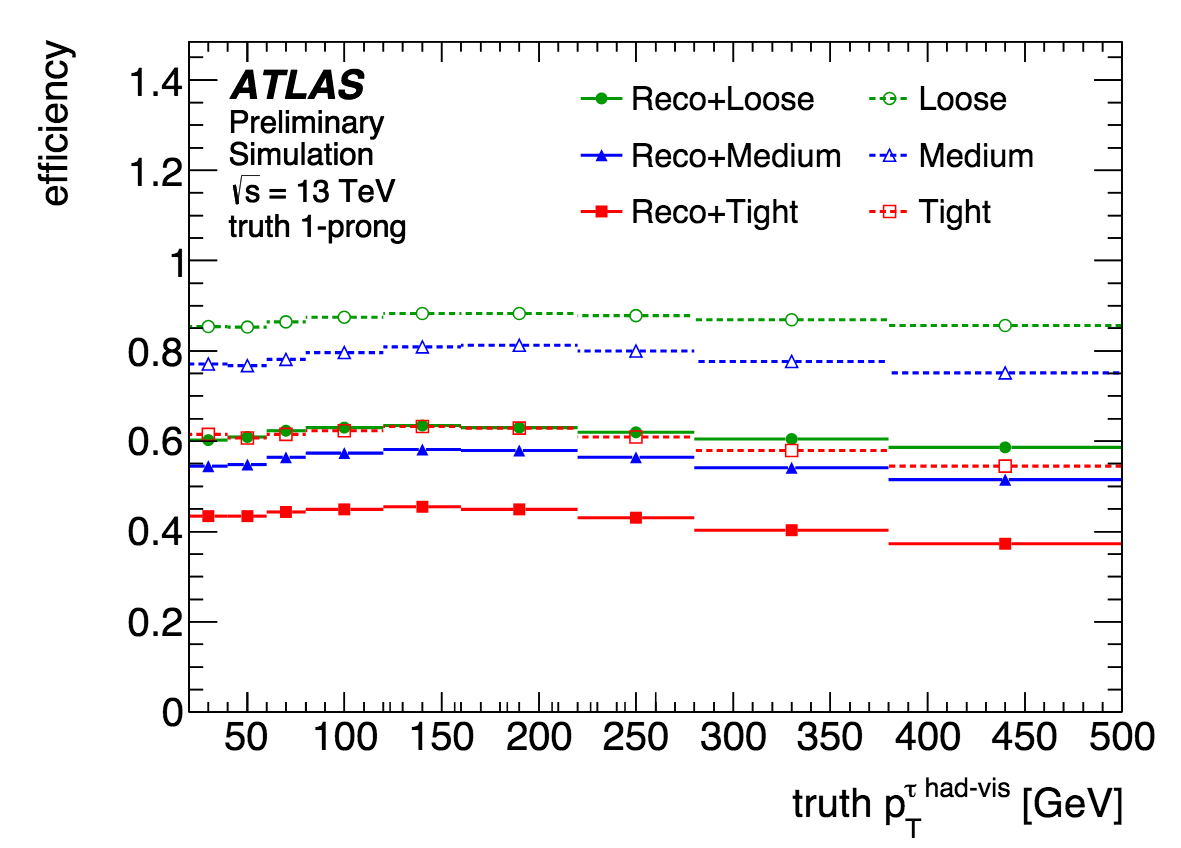
\includegraphics[width=2.5in]{figures/chapter3/tau_eff_1p.pdf}
    \end{subfigure}
    \begin{subfigure}
        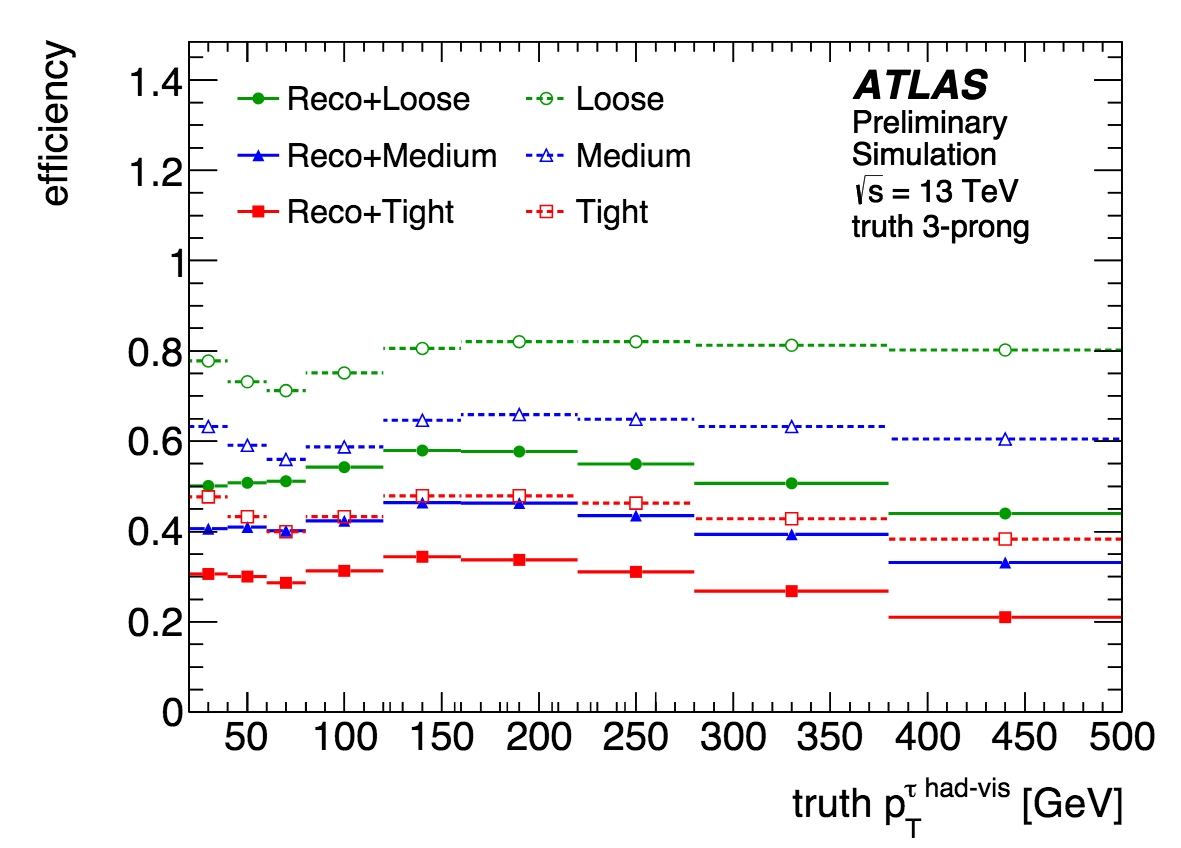
\includegraphics[width=2.5in]{figures/chapter3/tau_eff_3p.pdf}
    \end{subfigure}
    \caption{Efficiency for hadronic tau identification (open) and combined reconstruction and identification (closed) for one-prong (left) and three-prong (right) taus \cite{tau_id}.}
    \label{fig:tau_eff}
\end{figure}

%%met
\subsubsection{Missing Transverse Energy}
The law of conservation of momentum dictates that the net momentum in the transverse plane of a direct proton-proton collision should be zero. After reconstructing all tracks and objects in an event, any remaining momentum imbalance in the transverse plane is classified as missing transverse energy (MET). MET may be understood as indicating the presence of SM neutrinos, which are undetectable by ATLAS, or new BSM physics (also undetectable by ATLAS). However, it is important to also account for reconstruction and identification inefficiencies and other systematic effects.\\

The MET calculation is one of the more challenging reconstruction problems in ATLAS as it requires input from all detector subsystems and all other reconstruction and identification algorithms. The calculation combines contributions from hard objects (fully reconstructed and identified particles and jets) and soft signals (reconstructed charged particle tracks associated with the hard scatter primary vertex). The basic equation for calculating the components of MET is $$E_{x,(y)}^{miss}=-\sum_{i\epsilon\{\text{hard objects}\}}p_{x(y),i}-\sum_{j\epsilon\{\text{soft signals}\}}p_{x(y),j}.$$ This calculation requires that all contributing objects are reconstructed from mutually exclusive detector signals. Thus, overlapping reconstructed objects are rejected in a defined order; the most commonly used order is electrons, photons, taus, muons, jets, unused tracks, although this can be adjusted for different analysis requirements \cite{met_run2}. A demonstration of MET reconstruction performance is shown in Figure \ref{fig:met_eff}.\\

\begin{figure}[htb!]
    \centering
    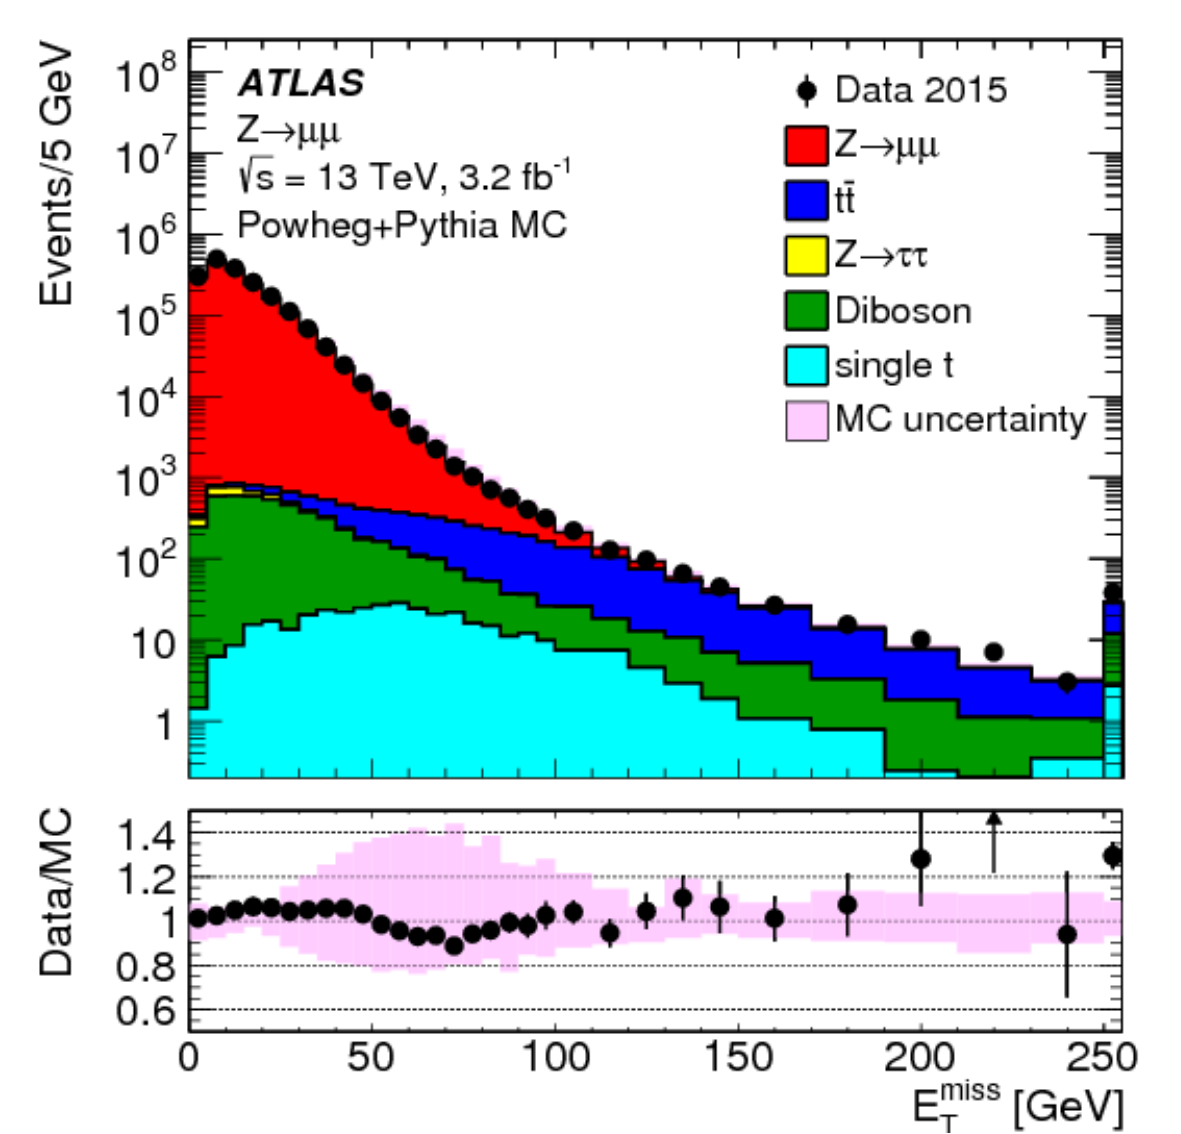
\includegraphics[width=4in]{figures/chapter3/met_eff.pdf}
    \caption{Distribution of MET for an inclusive sample of $Z\rightarrow\mu\mu$ events extracted from data and compared to MC \cite{met_run2}.}
    \label{fig:met_eff}
\end{figure}

%%subsec: Analyses
\subsection{Physics Analyses}
algorithm design, metric to fit, uncertainties, unblinding